\selectlanguage{french}
\Chapter{DISCUSSION GÉNÉRALE}\label{sec:Discussion}

\section{Autres travaux}

Les articles présentés dans le cadre de ce doctorat ne constituent qu'une portion de l'ensemble des travaux réalisés. 
Cette section présentera une partie de ces travaux supplémentaires. 

\subsection{Conception du montage de soudage par résistance}

Afin de pouvoir réaliser des essais de soudage, il a été nécessaire de concevoir et fabriquer un système de soudage par résistance. 
La conception du montage a nécessité de définir la géométrie du montage, le choix de la source, le système d'acquisition de données et l'interface de contrôle. 
Le système produit vise à être polyvalent et pourra servir à de nombreux projets de recherche. 

La polyvalence de la source a d'ailleurs été nécessaire après les premiers essais de soudage pour régler des problèmes de répétabilité. 
En raison de variations dans les dimensions des éléments chauffants et d'un mode de contrôle en voltage constant, la puissance dissipée dans les joints variait énormément d'un essai à l'autre. 
Développer le mode de contrôle en puissance constante a permis de stabiliser la quantité d'énergie dissipée dans le joint et d'obtenir des résultats répétables. 
Même lors d'essais de soudage avec des éléments chauffants en acier inoxydable, la variation de résistance causée par l'augmentation de température, ne vient plus affecter la quantité d'énergie dissipée. 

\subsection{Conception de l'élément chauffant nanocomposite}

La conception du nanocomposite et du montage de soudage ont été réalisés en parallèle. 
En se basant sur les puissances employées lors de soudages avec des éléments chauffants en acier inoxydable, ainsi qu'en fixant un voltage maximal, il a été possible d'établir une cible de conductivité de \SI{100}{\siemens\per\metre}. 

Afin d'atteindre cette cible, plusieurs compositions de nanocomposites ont été évaluées. 
Les charges conductrices sélectionnées pour ces essais étaient des nanotubes de carbone multi parois avec une pureté de 99\% et 95\%, des nanofibres de carbone ainsi que des nano plaquettes de graphène. 
Ces charges ont été mélangées à du PEI avec des fractions massiques allant jusqu'à 15\%.
La conductivité électrique des mélanges obtenus par extrusion a été évaluée à l'aide d'un système de mesure à 4 pointes. 
La figure \ref{fig:conductivite_lin} présente les résultats des mesures de conductivité électrique. 

\begin{figure}[h]
	\centering
	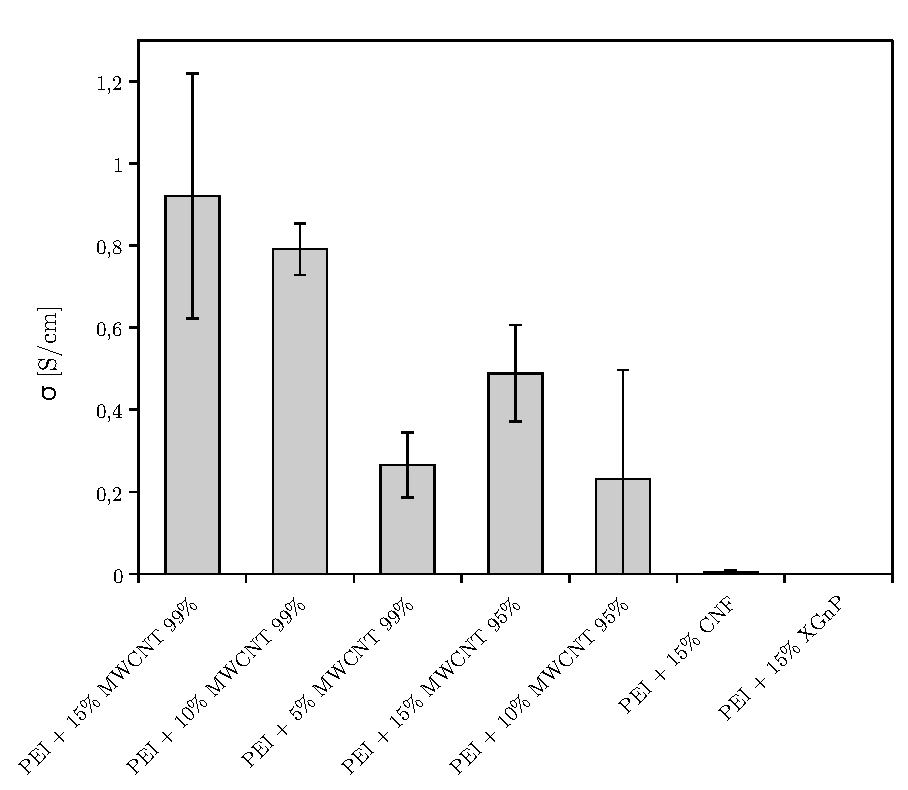
\includegraphics[width=0.75\textwidth]{conductivity_lin.pdf}
	\caption{Conductivité de mélanges de PEI et de particules conductrices}
	\label{fig:conductivite_lin}
\end{figure}

\FloatBarrier
\subsection{Résistance de contact des électrodes}

Dès le début des essais de soudage, des modèles simplifiés étaient développés en parallèle. 
En raison de divergence entre les mesures de température et les valeurs prévues lors des premiers essais, l'effet de la pression des électrodes contre le nanocomposite sur la résistance de contact a été évalué (Fig. \ref{fig:resistance_contact}). 
Une amélioration de la méthode de mesure de la résistance de contact, en isolant électriquement la section mesurée, a d'ailleurs été un élément clé pour l'élaboration du modèle présenté au chapitre \ref{sec:Theme2}. 

\begin{figure}[h]
	\centering
	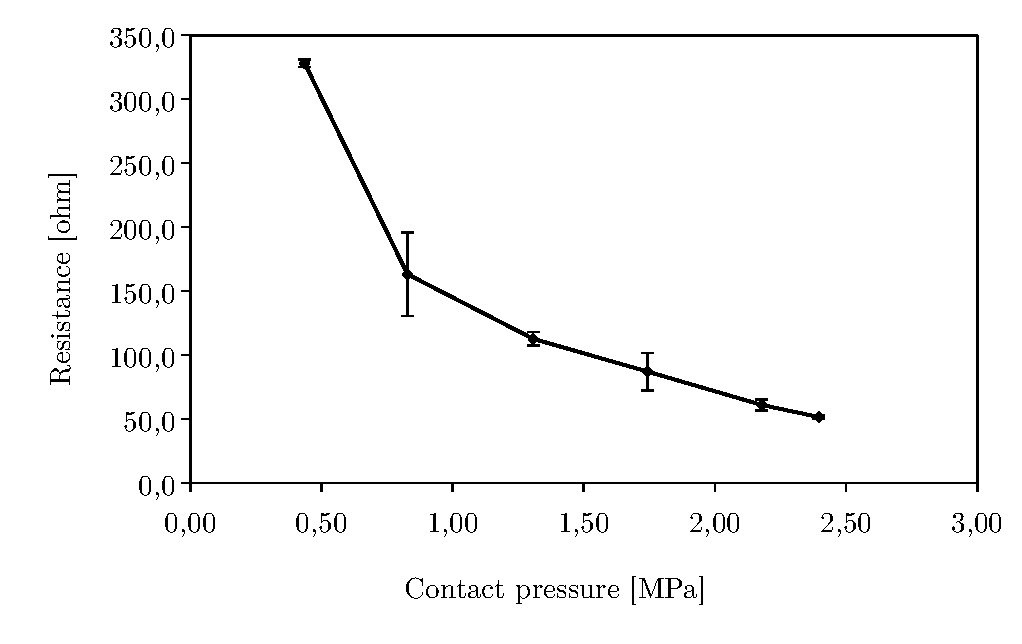
\includegraphics[width=0.75\textwidth]{contact_resistance.pdf}
	\caption{Effet de la pression sur la résistance de contact entre les électrodes de cuivre et le nanocomposite}
	\label{fig:resistance_contact}
\end{figure}

\FloatBarrier
\subsection{Analyse des porosités dans les joints}

Pour évaluer l'effet de la pression durant le soudage et pour assurer des joints de bonne qualité, des micrographies ont été prises afin d'identifier la présence de porosité (Fig. \ref{fig:micro_analyse_porosite}). 
Les échantillons pour ces observations ont produit depuis des tranches présentant le centre et le bord de la soudure. 

\begin{figure}[h!]
	\centering
	\subfigure[Absence de porosités]
	{\label{fig:micro_joint_sans_porosite} 								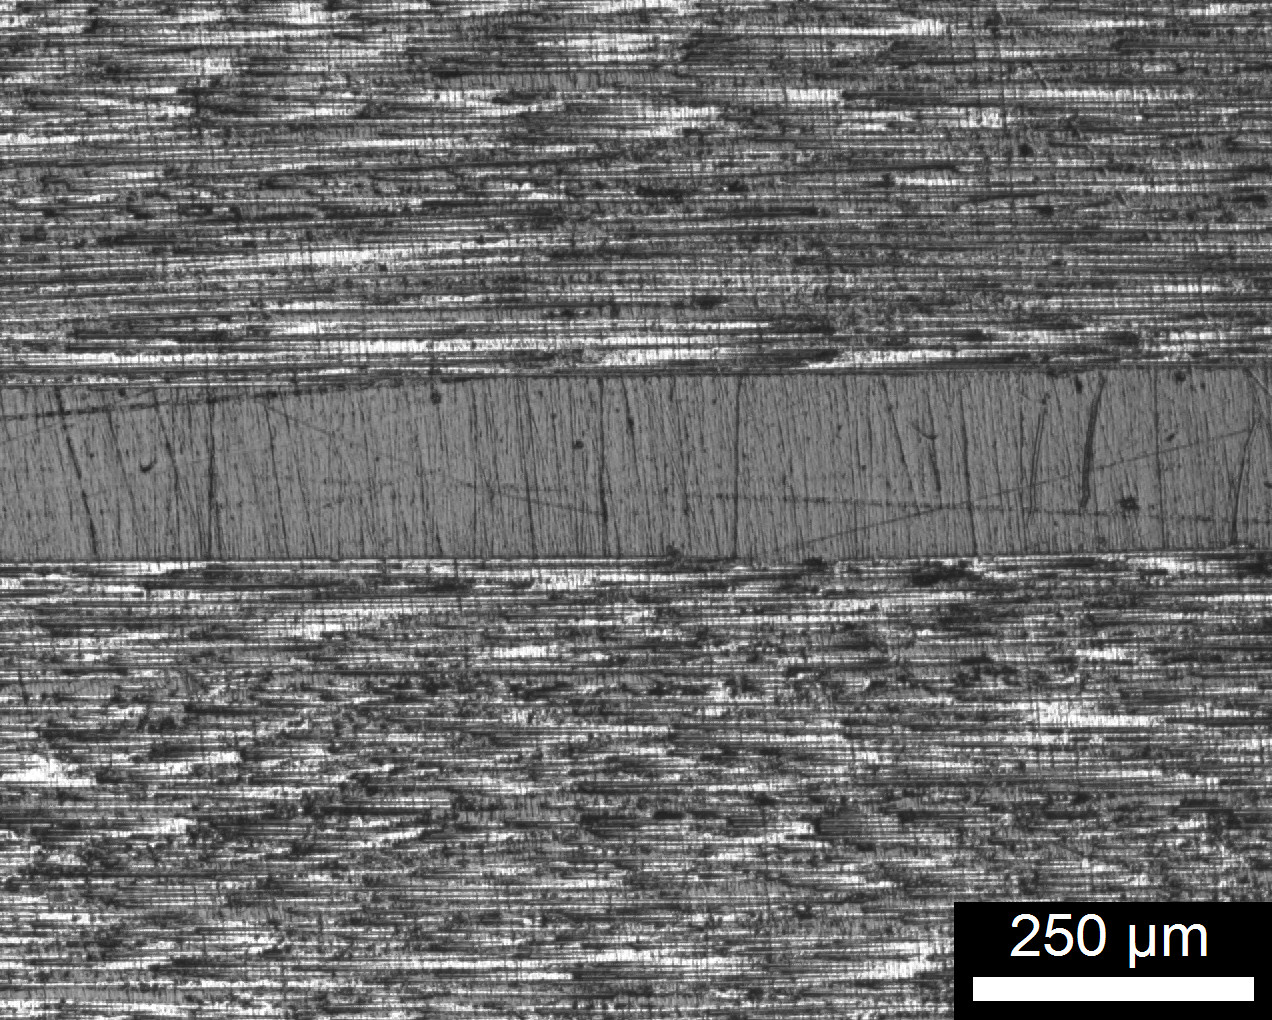
\includegraphics[width=0.45\textwidth]{0_6MPa_Milieu_01_bw.jpg}
	} \qquad
	\subfigure[Présence de porosités]
	{\label{fig:micro_joint_avec_porosite}
		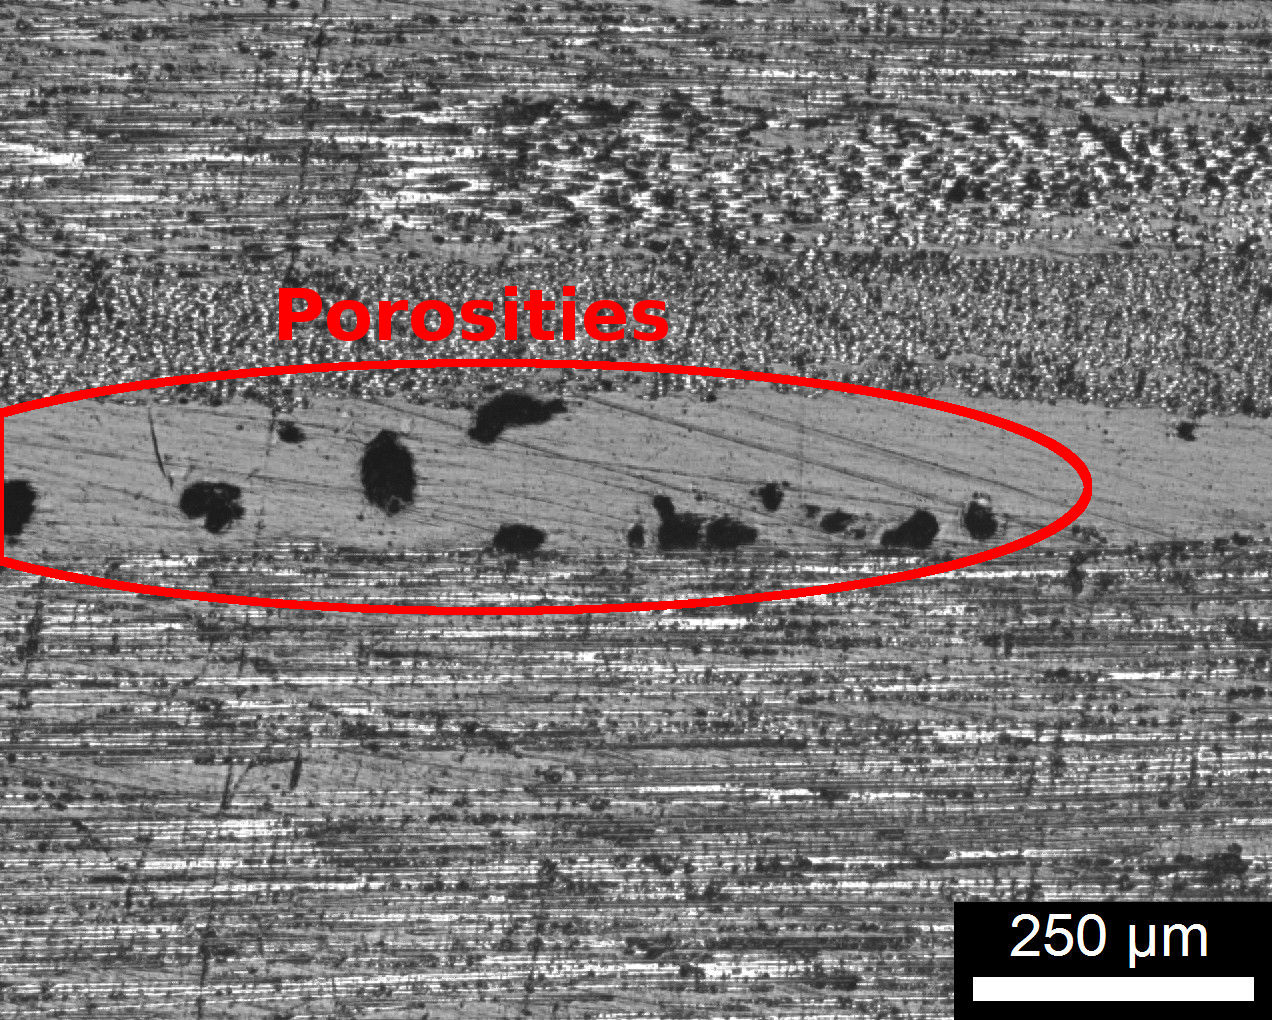
\includegraphics[width=0.45\textwidth]{1_4MPa_Milieu_02_bw_anotate.jpg}
	}
	\caption{Micrographies d'échantillons soudés ayant servi à l'analyse des porosités dans les joints}
	\label{fig:micro_analyse_porosite}
\end{figure}

\FloatBarrier
\section{Synthèse des travaux}

Les objectifs poursuivis dans le cadre de cette thèse se déclinaient comme suit : 

\begin{enumerate}
	\item Concevoir un élément chauffant nanocomposite conducteur en tenant compte des propriétés électriques et thermiques nécessaires au procédé de soudage par résistance. 
	\item Développer un procédé de soudage par résistance avec un élément chauffant nanocomposite entre deux adhérents en composite à matrice thermoplastique. 
	\item Établir une fenêtre d'opération pour le soudage par résistance avec un élément chauffant nanocomposite entre deux adhérents en composite à matrice thermoplastique. 
	\item Développer un procédé de soudage par résistance avec un élément chauffant nanocomposite entre un adhérent en composite à matrice thermoplastique et un adhérent en élastomère thermoplastique. 
\end{enumerate}

En premier lieu, un nanocomposite conducteur a été conçu et caractérisé. 
Pour ce faire, plusieurs compositions de nanocomposite ont été produites et évaluées. 
La composition démontrant les meilleures caractéristiques a été produite en plus grande quantité et utilisée pour démontrer la possibilité de l'utiliser comme élément chauffant. 
La preuve de concept du procédé de soudage utilisant ce nanocomposite a permis de valider le concept d'un élément chauffant nanocomposite. 

En second lieu, un modèle par éléments finis a été développé afin d'établir les limites de la fenêtre d'opération du procédé de soudage. 
Des essais de soudage supplémentaires en laboratoire sont venus confirmer la fenêtre identifiée. 
Grâce à un meilleur contrôle du procédé, il a été possible d'améliorer les performances mécaniques des joints. 

Finalement, la production de jonctions soudées flexibles à l'aide du procédé de soudage résistif a été explorée et quelques avancées ont été obtenues. 
Cette exploration a mené à la sélection du ULTEM STM1500 qui est compatible avec le PEI. 
Par contre, les travaux de cette thèse n'ont cependant pas permis de trouver des paramètres opérationnels permettant d'obtenir un soudage multi matériau rencontrant les requis techniques d'ArianeGroup. 
Certaines pistes supplémentaires ont été identifiées telles que le taux d'humidité dans le nanocomposite et l'élastomère ainsi que la possibilité de texturer le nanocomposite. 

Les objectifs 1 à 3 ont été couverts et atteints par les articles présentés aux chapitres \ref{sec:Theme1} et \ref{sec:Theme2}. 
Le premier article \cite{Brassard2019a} a été publié en février 2019 dans la revue \textit{Composites Part B: Engineering} après révision par les pairs. 
Cet article a déjà été reconnu et cité par d'autres chercheurs travaillant au développement de nouveaux éléments chauffants pour le soudage des composites à matrice thermoplastique \cite{Russello2019}. 
Le second article a été soumis au journal \textit{Composites Part B: Engineering} en octobre 2019 et est en attente de révision par les pairs. 
En ce qui concerne l'objectif 4, ce dernier fait l'objet du chapitre \ref{sec:Theme3}. 